\documentclass[compress]{beamer}
\usepackage{ifthen,verbatim}

\newcommand{\isnote}{}
\xdefinecolor{lightyellow}{rgb}{1.,1.,0.25}
\xdefinecolor{darkblue}{rgb}{0.1,0.1,0.7}

%% Uncomment this to get annotations
%% \def\notes{\addtocounter{page}{-1}
%%            \renewcommand{\isnote}{*}
%% 	   \beamertemplateshadingbackground{lightyellow}{white}
%%            \begin{frame}
%%            \frametitle{Notes for the previous page (page \insertpagenumber)}
%%            \itemize}
%% \def\endnotes{\enditemize
%% 	      \end{frame}
%%               \beamertemplateshadingbackground{white}{white}
%%               \renewcommand{\isnote}{}}

%% Uncomment this to not get annotations
\def\notes{\comment}
\def\endnotes{\endcomment}

\setbeamertemplate{navigation symbols}{}
\setbeamertemplate{headline}{\mbox{ } \hfill
\begin{minipage}{5.5 cm}
\vspace{-0.75 cm} \small
\end{minipage} \hfill
\begin{minipage}{4.5 cm}
\vspace{-0.75 cm} \small
\begin{flushright}
\ifthenelse{\equal{\insertpagenumber}{1}}{}{Jim Pivarski \hspace{0.2 cm} \insertpagenumber\isnote/\pageref{numpages}}
\end{flushright}
\end{minipage}\mbox{\hspace{0.2 cm}}\includegraphics[height=1 cm]{../cmslogo} \hspace{0.1 cm} \includegraphics[height=1 cm]{../tamulogo} \hspace{0.01 cm} \vspace{-1.05 cm}}

\begin{document}
\begin{frame}
\begin{center}
\vfill \textcolor{darkblue}{\LARGE Muon Alignment: Endcaps}

\vspace{0.5 cm} \small Joint DPG and Physics Muon Workshop, 3 April 2008

\vfill \begin{tabular}{c c c}
\textcolor{darkblue}{Jim Pivarski} & & \textcolor{darkblue}{Samir Guragain} \\
\textcolor{darkblue}{Alexei Safonov} & \textcolor{darkblue}{K\'aroly Banicz} & \textcolor{darkblue}{Marcus Hohlmann} \\
\small Texas A\&M University & \small FermiLab & \small Florida Inst.\ of Technology
\end{tabular}

\end{center}
\end{frame}

%% \begin{notes}
%% \item This is the annotated version of my talk.
%% \item If you want the version that I am presenting, download the one
%% labeled ``slides'' on Indico (or just ignore these yellow pages).
%% \item The annotated version is provided for extra detail and a written
%% record of comments that I intend to make orally.
%% \item Yellow notes refer to the content on the {\it previous} page.
%% \item All other slides are identical for the two versions.
%% \end{notes}

\begin{frame}
\frametitle{CSC Alignment Outline}
\large
\begin{itemize}\setlength{\itemsep}{0.5 cm}
\item Hardware alignment
\item Track-based alignment

\begin{itemize}\setlength{\itemsep}{0.3 cm}
\item \large Baseline and start-up procedures
\item \large iCSA08 exercise
\end{itemize}
\item Hardware/track-based comparisons
\item Timelines
\end{itemize}
\end{frame}

\begin{frame}
\frametitle{Hardware alignment}
\large
\begin{itemize}\setlength{\itemsep}{0.2 cm}
\item ME+2 DCOPS alignment finalized in MTCC \\ (field on and off)
\item Comparison with photogrammetry in 0T to test accuracy (next two slides)
\item Observed expected deformations from 0T to 4T
\begin{center}
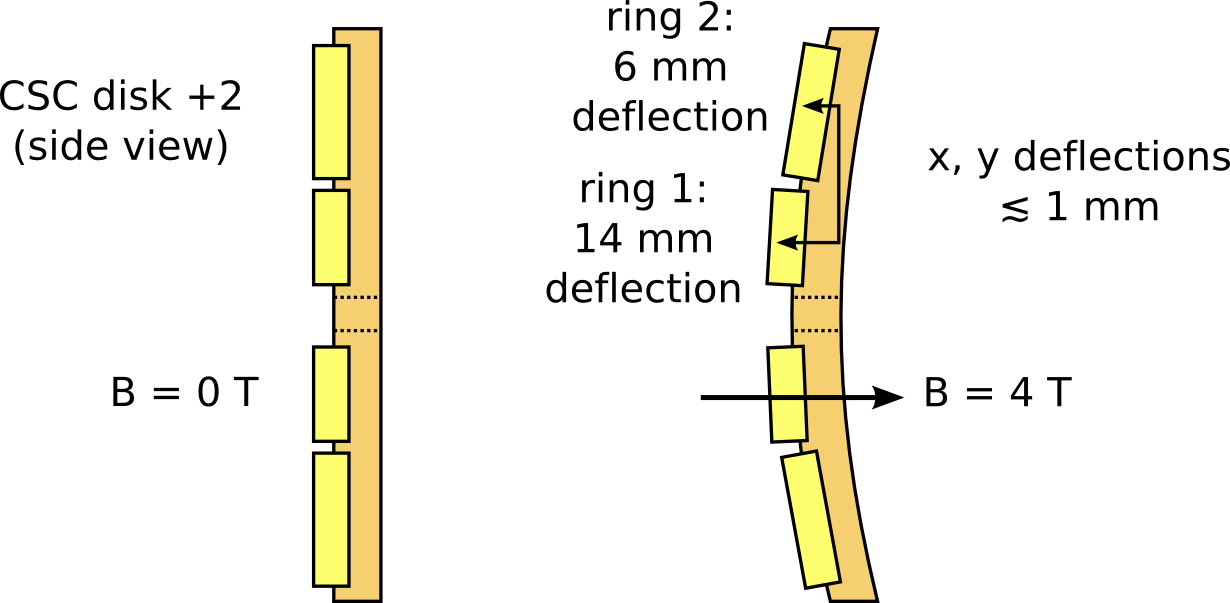
\includegraphics[width=0.8\linewidth]{deflections.png}
\end{center}
\item Now Samir and Marcus are working on other stations
\end{itemize}
\end{frame}

\begin{frame}
\mbox{\hspace{-1 cm}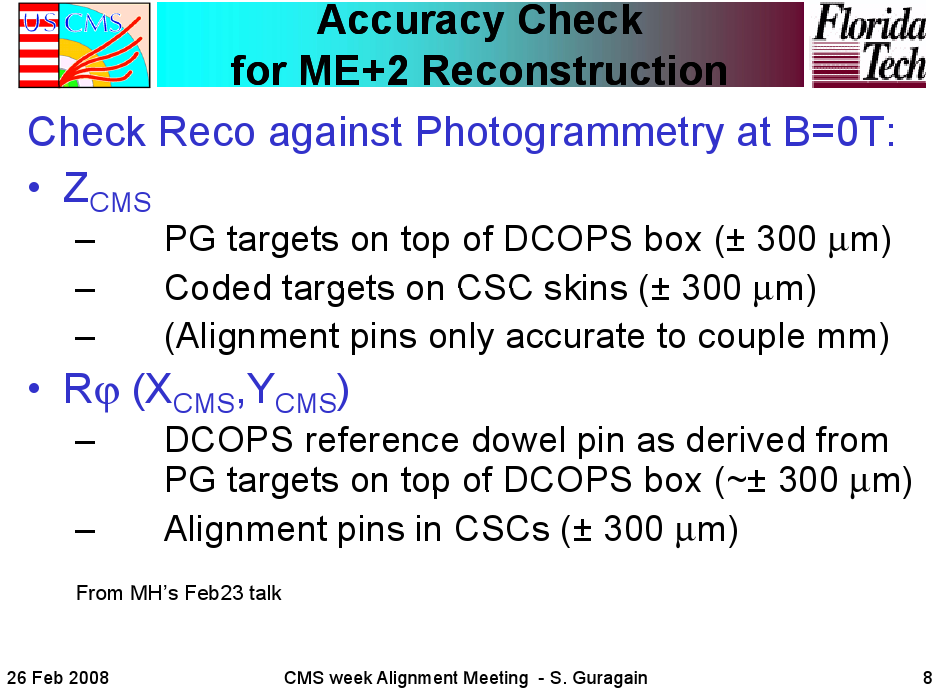
\includegraphics[width=1.2\linewidth]{samirs_plots2.png}}
\end{frame}

\begin{frame}
\mbox{\hspace{-1 cm}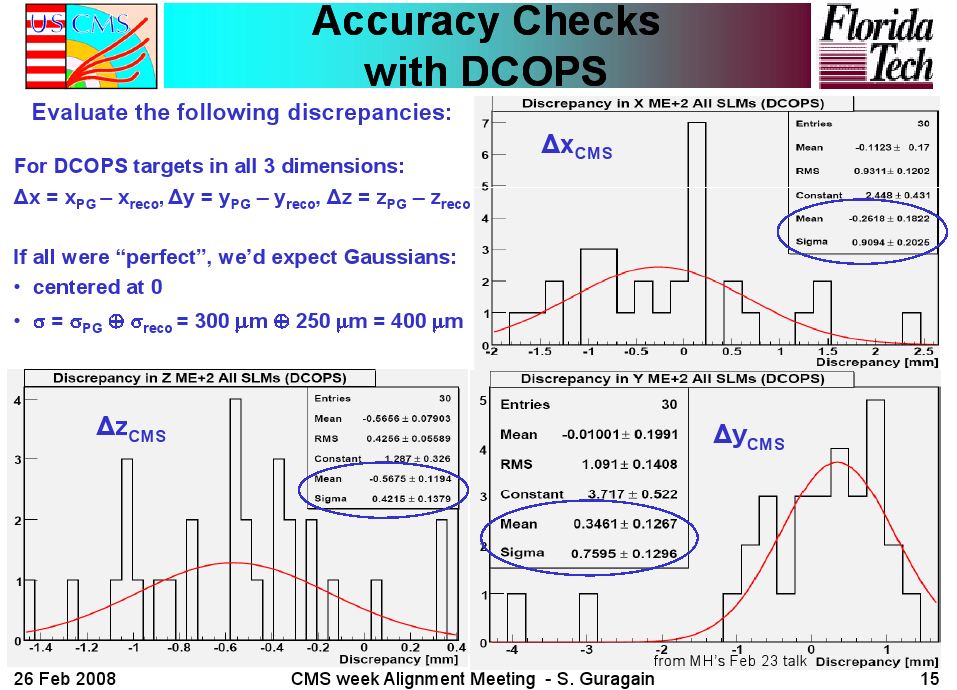
\includegraphics[width=1.2\linewidth]{samirs_plots.png}}
\end{frame}

\begin{frame}
\frametitle{Track-based alignment}

\vspace{2.2 cm}
\hfill 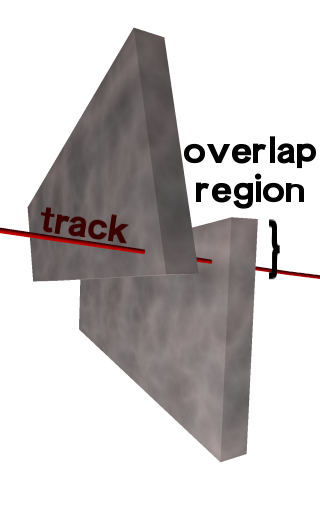
\includegraphics[width=0.15\linewidth]{overlap.png}

\vspace{-5 cm}
\begin{itemize}\setlength{\itemsep}{0.3 cm}
\item \textcolor{darkblue}{\large Baseline HIP procedure}
\begin{itemize}
\item whole muon system (CSCs {\it and} DTs)
\item uses silicon tracker as an external reference
\item requires at least 10~pb$^{-1}$
\item well-studied procedure
\end{itemize}

\item \textcolor{darkblue}{\large CSC overlap procedure}
\begin{itemize}
\item tracks through overlap regions measure relative \\ alignment of pairs of neighboring chambers
\item all CSC chambers except ME1/3 have overlap regions
\end{itemize}

\vspace{-0.25 cm}
\begin{enumerate}
\item optimize alignment within each CSC ring
\item follow-up by aligning each CSC ring to tracker (very easy)
\end{enumerate}

\item \textcolor{darkblue}{\large CSC layer procedure}
\begin{itemize}
\item align CSC layers relative to layer 1 (similar to above)
\end{itemize}
\end{itemize}

% \small
\vspace{0.2 cm} \textcolor{darkblue}{Overlap} and \textcolor{darkblue}{layer}
procedures can be done with low-momentum I.P.\ muons or beam-halo

%% \vspace{0.15 cm} If beam-halo rate is high enough (far enough from the
%% beamline), we could align all layers and all chambers except ME1/3 before first collisions
\end{frame}

\begin{frame}
\frametitle{Baseline procedure}

\begin{itemize}
\item Tracks are iteratively re-fit with varying hit-weights
\begin{enumerate}
\item loose hit weights in the muon system: project tracks from tracker and align first station
\item tight hit weights in first station: align second station
\item etc.
\end{enumerate}
\item Each chamber is aligned independently of its neighbors
\end{itemize}

\vfill
\begin{columns}
\column{0.6\linewidth}
\begin{itemize}\setlength{\itemsep}{0.25 cm}
\item Test in CRAFT: full tracker and high statistics for top and bottom chambers

\item Maybe test in CRA0T: how essential is our $p_T$ cut? \mbox{(to be studied)\hspace{-1 cm}}

\item Estimate 1~million \mbox{muons in MB0 (good),\hspace{-2 cm}} \\ 10k muons in ME1/3 (fair)
\end{itemize}

\vspace{0.3 cm}\mbox{ }

\column{0.5\linewidth}
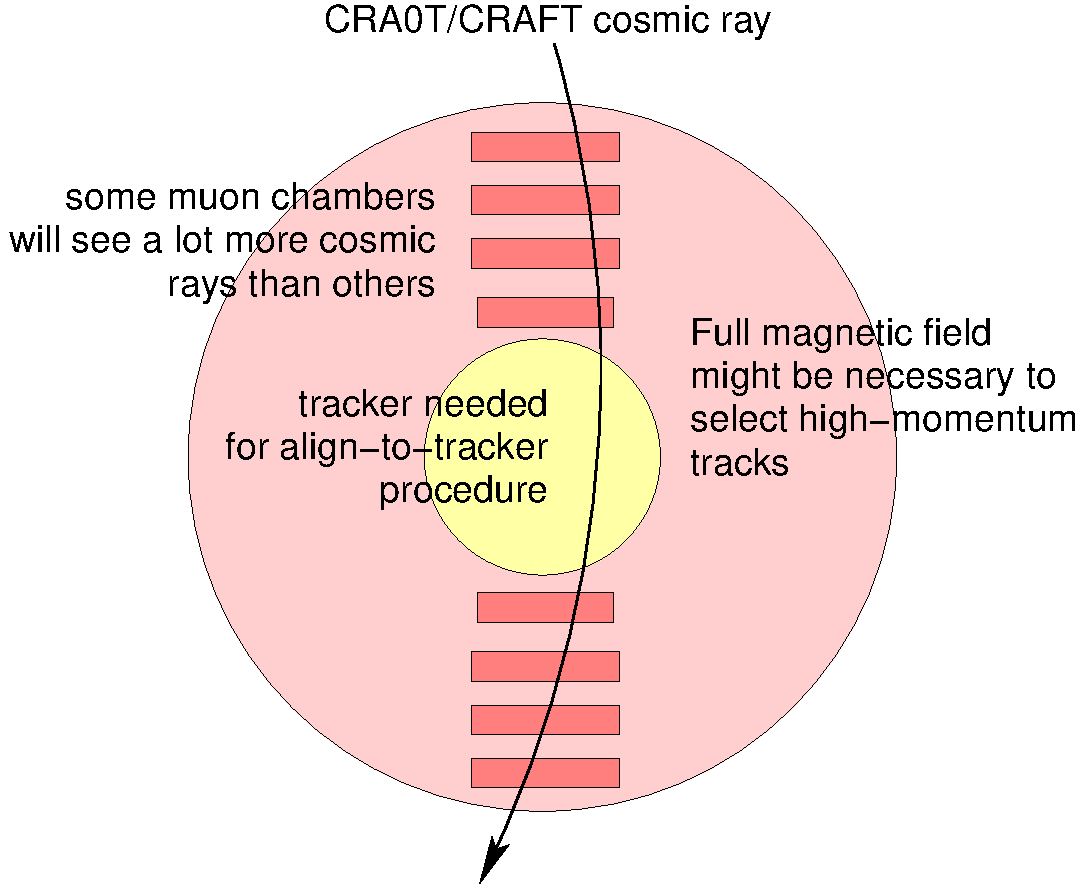
\includegraphics[width=\linewidth]{craft.pdf}
\end{columns}
\end{frame}

\begin{frame}
\frametitle{Beam-halo procedures}

\vspace{-0.5 cm}
\begin{center}
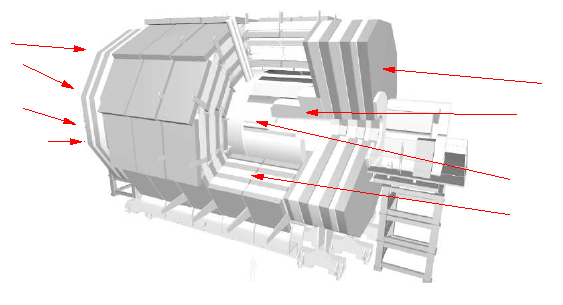
\includegraphics[height=3 cm]{beam-halo_schematic.png} 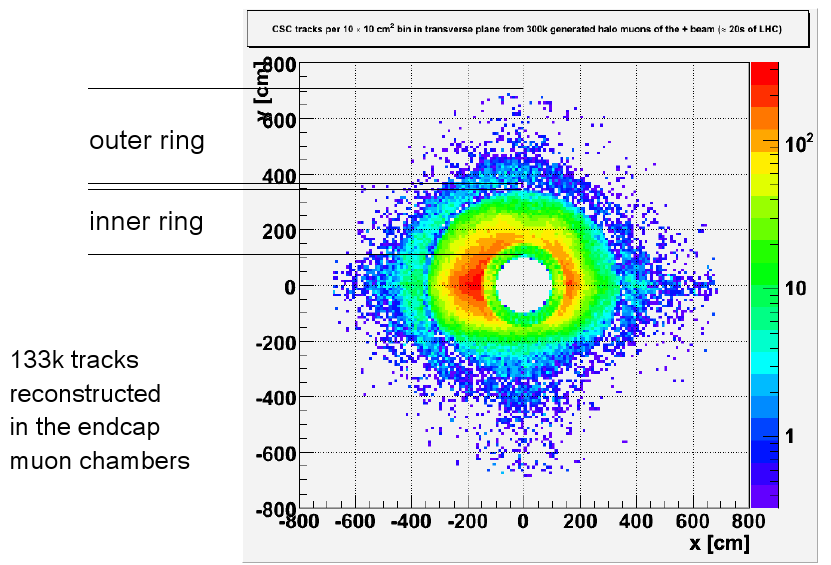
\includegraphics[height=4 cm]{beam-halo.png}
\end{center}

\begin{itemize}
\item Beam-halo may be a good source of horizontal muons before first collisions
\item Rate is very uncertain (simulation suggests we'll have enough
muons, but uncertainty quoted as factor of 100)
\item Same techniques can be applied to low-energy I.P.\ muons
\end{itemize}

\end{frame}

\begin{frame}
\frametitle{iCSA08 challenge}

Realistic alignment exercise in real-time

\begin{itemize}\setlength{\itemsep}{0.2 cm}
\item Baseline alignment (10~pb$^{-1}$) \textcolor{darkblue}{(minimal goal)}
\item CSC overlaps alignment (1 or 10~pb$^{-1}$, beam-halo)
\item CSC layer alignment (1 or 10~pb$^{-1}$, beam-halo)
\end{itemize}

\vfill All workflows will be pre-tested

\begin{itemize}\setlength{\itemsep}{0.2 cm}
\item iCSA08 conducted in CMSSW\_2\_0\_X
\item Back-ported new features to 1\_6\_7 and 1\_8\_X, to test with old CSA07 samples and new FastSim samples
\end{itemize}

\vfill Determined resource requirements for baseline procedure, others are in progress
\end{frame}

\begin{frame}
\frametitle{Alignment comparisons}

\begin{columns}
\column{0.8\linewidth}
Hardware/track-based alignments measure some parameters in common, others are orthogonal

\begin{center}
\begin{minipage}{0.8\linewidth}
Example:
\begin{itemize}
\item tracks measure CSC $x$, $y$
\item DCOPS measure CSC $x$, $z$
\end{itemize}

agreement in $x$ lends credence to $z$
\end{minipage}
\end{center}

\column{0.2\linewidth}
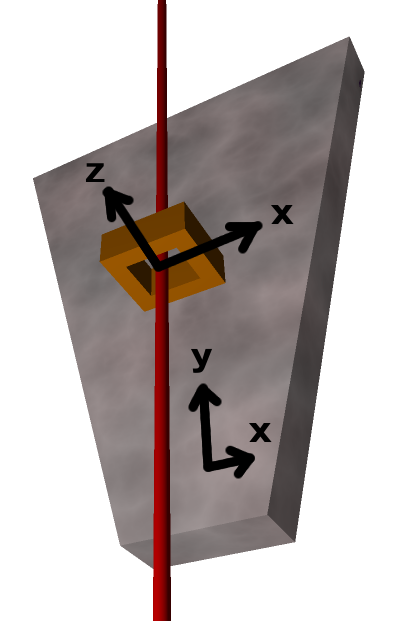
\includegraphics[width=\linewidth]{comparison.png}
\end{columns}

\vfill
But we need to measure the same dataset

\vspace{0.25 cm}
\mbox{\small \hspace{-0.75 cm} \renewcommand{\arraystretch}{1.4} \begin{tabular}{l p{0.28\linewidth} p{0.5\linewidth}}
& \textcolor{darkblue}{hardware alignment} & \hfill \textcolor{darkblue}{track-based alignment} \hfill \mbox{ } \\\hline\hline
MTCC & done for ME+2 & possible testing-ground for beam-halo, if there is time \\
\mbox{CRA0T/CRAFT\hspace{-0.25 cm}} & barrel, link, ME1/3

proximity sensors? & top and bottom chambers in barrel, possibly ME1/3 if enough events \\
single-beam & full endcap \mbox{procedure\hspace{-0.25 cm}} & ring 1 well-measured, ring 2 less so \\\hline
\end{tabular}}
\end{frame}

\begin{frame}
\frametitle{Timelines}

\vspace{0.5 cm} \mbox{\hspace{-0.75 cm}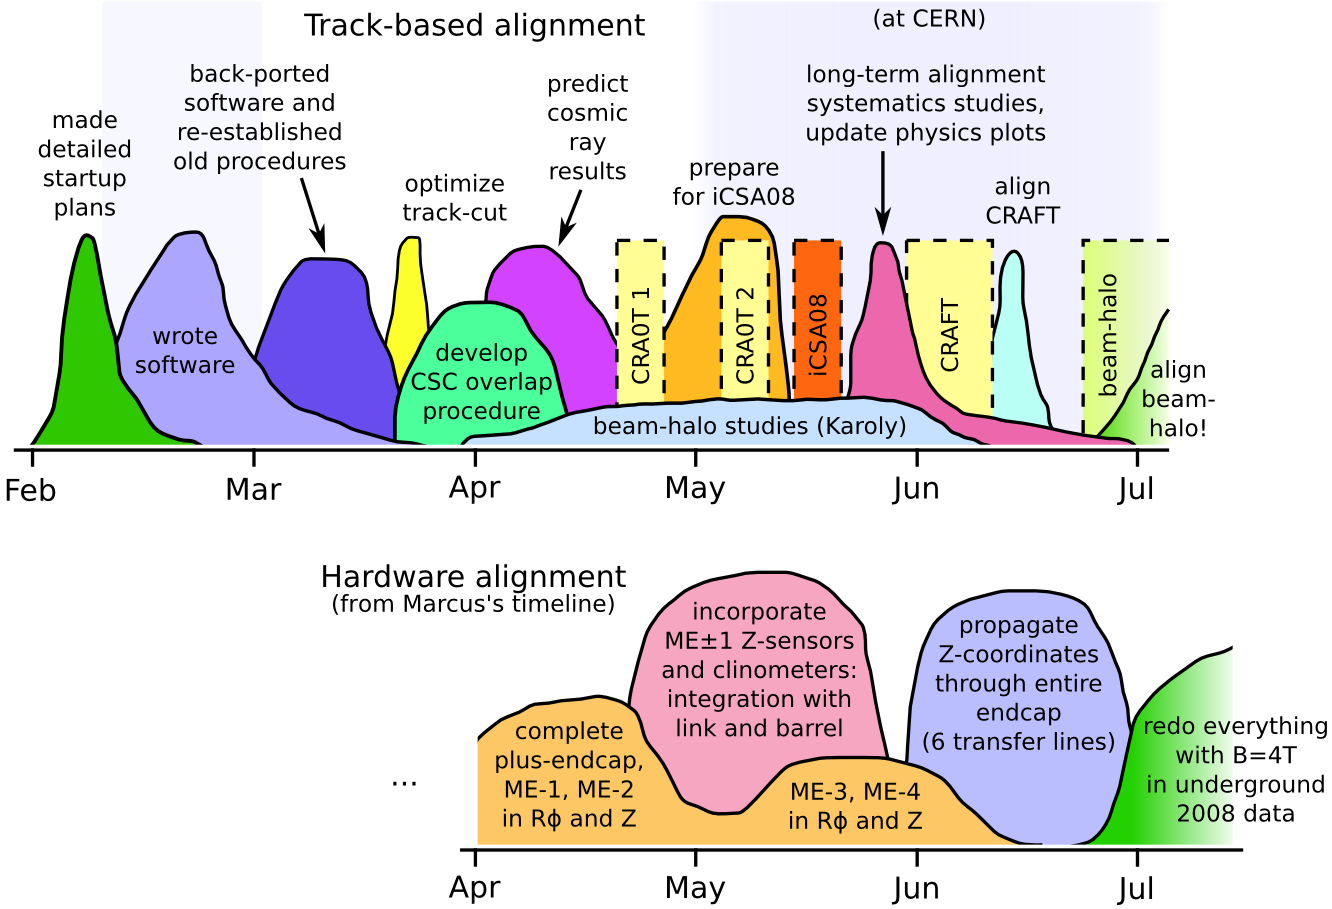
\includegraphics[width=1.1\linewidth]{plan.png}}
\end{frame}


\begin{frame}
\frametitle{Conclusions}
\large
\begin{itemize}\setlength{\itemsep}{0.5 cm}
\item Hardware alignment is producing sensible results in MTCC
\item Baseline procedure for whole muon system in good shape
\item Start-up procedures for endcap in development
\item These will be tested in iCSA08
\item Likely date for comparisons: June or July
\end{itemize}
\label{numpages}
\end{frame}

%% \begin{frame}
%% \frametitle{Outline}
%% \begin{itemize}\setlength{\itemsep}{0.75 cm}
%% \item 
%% \end{itemize}
%% %% \hspace{-0.83 cm} \textcolor{darkblue}{\Large Outline2}
%% \end{frame}

%% %% \section*{First section}
%% %% \begin{frame}
%% %% \begin{center}
%% %% \Huge \textcolor{blue}{First section}
%% %% \end{center}
%% %% \end{frame}

\end{document}
